\documentclass[12pt,a4paper]{article}

% -----------------------------------------------------
% PACKAGES
% -----------------------------------------------------
\usepackage[utf8]{inputenc}
\usepackage[T1]{fontenc}

\usepackage{amsmath,amssymb,amsfonts,mathrsfs}
\usepackage{tikz}
\usetikzlibrary{patterns,arrows,shapes.geometric,fit}

\usepackage{enumitem}
\usepackage{multicol}
\usepackage{lmodern}
\usepackage{times}
\usepackage{pifont}

\usepackage[left=1cm,right=1cm,top=1cm,bottom=1.7cm]{geometry}

\usepackage[colorlinks=true, linkcolor=blue, urlcolor=blue, citecolor=blue]{hyperref}

\usepackage{array,multirow}
\usepackage[most]{tcolorbox}
\tcbuselibrary{skins,hooks}

\usepackage{varwidth}
\usepackage{float}

\usepackage{fancyhdr}
\usepackage{eso-pic}

\usepackage{tkz-tab}
\usepackage{systeme}
\usepackage{verbatim}
\usepackage{color,soul}

% -----------------------------------------------------
% TEXTE EN ARRIÈRE-PLAN (1 seule fois)
% -----------------------------------------------------
\AddToShipoutPicture{
    \AtTextCenter{%
        \makebox[0pt]{\rotatebox{80}{\textcolor[gray]{0.7}{\fontsize{5cm}{5cm}\selectfont PGB}}}
    }
}

% -----------------------------------------------------
% COMMANDES PERSONNALISÉES
% -----------------------------------------------------

% Items
\newcommand\circitem[1]{%
\tikz[baseline=(char.base)]{
\node[circle,draw=gray, fill=red!55,
minimum size=1.2em,inner sep=0] (char) {#1};}}

\newcommand\boxitem[1]{%
\tikz[baseline=(char.base)]{
\node[fill=cyan,
minimum size=1.2em,inner sep=0] (char) {#1};}}

\setlist[enumerate,1]{label=\protect\circitem{\arabic*}}
\setlist[enumerate,2]{label=\protect\boxitem{\alph*}}

\everymath{\displaystyle}

% EXEMPLES
\newcounter{exemple}
\newcommand{\exemple}{%
  \refstepcounter{exemple}%
  \textbf{\textcolor{green}{Exemple \theexemple :}} \ignorespaces
}

% EXERCICES D’APPLICATION
\definecolor{myorange}{rgb}{1.0, 0.8, 0.0}

\newcounter{exerciceapp}
\newcommand{\exerciceapp}{%
  \refstepcounter{exerciceapp}%
  \textbf{\textcolor{myorange}{Exercice d'application \theexerciceapp :}} \ignorespaces
}

% CORRECTIONS
\newcounter{correction}
\newcommand{\correction}{%
  \refstepcounter{correction}%
  \textbf{\textcolor{myorange}{Correction \thecorrection :}} \ignorespaces
}

% Soulignement coloré
\newcommand{\myul}[2][black]{\setulcolor{#1}\ul{#2}\setulcolor{black}}

% Tabulation
\newcommand\tab[1][1cm]{\hspace*{#1} }

% -----------------------------------------------------
% DOCUMENT
% -----------------------------------------------------
\begin{document}

\begin{center}
    \Large\textbf{\underline{Dérivabilité et Applications}}\\[-0.1cm]
    \normalsize\textbf{Prof : M. BA} \hfill \textbf{Classe : 1erL}\\[-0.1cm]
    \textbf{Année scolaire : 2025 -- 2026}
\end{center}

\section*{Introduction à la notion de dérivation}
L'objectif du calcul différentiel en classe de Littéraire est principalement d'étudier les variations d'une fonction (savoir si elle monte ou descend) et de résoudre des problèmes d'optimisation (recherche d'un bénéfice maximal par exemple).

\section*{I.\quad Nombre dérivé en un point}

\subsection*{1)\quad Taux de variation d'une fonction}

\subsubsection*{a)\quad Approche et calcul}

Soit $f$ la fonction définie sur $\mathbb{R}$ par $f(x)=x^2$. Prenons un point fixe d'abscisse $1$. Choisissons des valeurs de $x$ de plus en plus proches de $1$ et calculons le rapport $\frac{f(x)-f(1)}{x-1}$ appelé taux de variation :

\begin{center}
\begin{tabular}{|c|c|c|c|c|c|}
\hline
$x$ & $1{,}1$ & $1{,}01$ & $1{,}001$ & $0{,}99$ & $0{,}999$ \\
\hline
$f(x) = x^2$ & $1{,}21$ & $1{,}0201$ & $1{,}002001$ & $0{,}9801$ & $0{,}998001$ \\
\hline
$\frac{f(x)-f(1)}{x-1}$ & $2{,}1$ & $2{,}01$ & $2{,}001$ & $1{,}99$ & $1{,}999$ \\
\hline
\end{tabular}
\end{center}

\bigskip

\begin{center}
\textbf{Exploitation}
\end{center}

D'après le tableau ci-dessus, on constate que si les valeurs de $x$ se rapprochent de $1$, le taux de variation se rapproche de la valeur unique $2$.

On dit que la fonction $f$ est dérivable en $1$ et que son nombre dérivé en $1$ est égal à $2$.

On note :
\[
f'(1) = 2
\]

\subsubsection*{b)\quad Définition générale et notation}

Soit $f$ une fonction définie sur un intervalle $I$ et $a$ un nombre réel appartenant à $I$.\\
On dit que $f$ est dérivable en $a$ si le taux de variation $\frac{f(x)-f(a)}{x-1}$ se rapproche d'un nombre réel fixe $l$ lorsque $x$ tend vers $a$.

Ce nombre réel $l$ est appelé \textbf{nombre dérivé de $f$ en $a$} et est noté $\boxed{f'(a)}$.
\[
\lim_{x \to a} \frac{f(x)-f(a)}{x-a} = f'(a)
\]

\bigskip

\subsubsection*{c)\quad Interprétation géométrique : La Tangente}
\textbf{Propriété :} Le nombre dérivé $f'(a)$ est le coefficient directeur (la pente) de la droite tangente à la courbe de $f$ au point d'abscisse $a$.

\textbf{Équation de la tangente :} 
La tangente à la courbe de $f$ au point d'abscisse $a$ a pour équation :
\[
y = f'(a)(x-a) + f(a)
\]

\bigskip

\checkmark\ \exemple 

Soit la fonction $f(x) = x^2$ pour laquelle on sait que $f(1)=1$ et $f'(1)=2$. 
Déterminons l'équation de la tangente à sa courbe représentative au point d'abscisse $1$.

D'après la formule, on a :
\[
y = f'(1)(x-1) + f(1)
\]
\[
y = 2(x-1) + 1
\]
\[
y = 2x - 2 + 1
\]
\[
\boxed{y = 2x - 1}
\]

\subsection*{2)\quad Fonction dérivée d'une fonction}

\subsubsection*{a)\quad Notion de fonction dérivée}

Lorsque qu'une fonction est dérivable en tout point d'un intervalle, on peut associer à chaque réel $x$ son nombre dérivé $f'(x)$. Cette nouvelle fonction s'appelle la \textbf{fonction dérivée} et se note $f'$.

\subsubsection*{b)\quad Formules des dérivées des fonctions usuelles}

\begin{center}
\begin{tabular}{|c|c|c|}
\hline
\textbf{Fonction } $f(x)$ & \textbf{Domaine de définition} & \textbf{Dérivée } $f'(x)$ \\
\hline
$k$ \small{(constante)} & $\mathbb{R}$ & $0$ \\
\hline
$x$ & $\mathbb{R}$ & $1$ \\
\hline
$ax+b$ & $\mathbb{R}$ & $a$ \\
\hline
$x^2$ & $\mathbb{R}$ & $2x$ \\
\hline
$x^3$ & $\mathbb{R}$ & $3x^2$ \\
\hline
$\frac{1}{x}$ & $\mathbb{R}^*$ & $-\frac{1}{x^2}$ \\
\hline
\end{tabular}
\end{center}

\bigskip

\checkmark\ \exemple
\begin{enumerate}
    \item Soit $f(x) = 7$ (fonction constante), alors $\boxed{f'(x) = 0}$.
    \item Soit $f(x) = 4x - 3$, alors $\boxed{f'(x) = 4}$.
    \item Soit $f(x) = x^2$, alors sa dérivée en $x = 5$ est $f'(5) = 2 \times 5 = \boxed{10}$.
\end{enumerate}

\bigskip

\subsubsection*{c)\quad Généralisation : Formules des dérivées d'opérations}

Voici les formules pour les cas généraux où $u$ et $v$ sont deux fonctions dérivables :

\begin{center}
\begin{tabular}{|c|c|c|}
\hline
\textbf{Opération} & \textbf{Fonction} & \textbf{Dérivée} \\
\hline
Puissance & $u^n$ & $n \cdot u' \cdot u^{n-1}$ \\
\hline
Quotient & $\frac{u}{v}$ \small{($v \neq 0$)} & $\frac{u'v - uv'}{v^2}$ \\
\hline
Racine carrée & $\sqrt{u}$ \small{($u > 0$)} & $\frac{u'}{2\sqrt{u}}$ \\
\hline
\end{tabular}
\end{center}

\bigskip

\checkmark\ \exemple
Soit la fonction $f$ définie sur $\mathbb{R} \setminus \{-2\}$ par :
\[
f(x) = \frac{2x + 1}{x + 2}
\]
Calculons sa fonction dérivée $f'$ en utilisant la formule du quotient $\frac{u}{v}$.

On pose :
\begin{itemize}
    \item $u(x) = 2x + 1 \implies u'(x) = 2$
    \item $v(x) = x + 2 \implies v'(x) = 1$
\end{itemize}

En appliquant la formule $\frac{u'v - uv'}{v^2}$, on obtient :
\[
f'(x) = \frac{2(x + 2) - (2x + 1)(1)}{(x + 2)^2}
\]
\[
f'(x) = \frac{2x + 4 - 2x - 1}{(x + 2)^2}
\]
\[
\boxed{f'(x) = \frac{3}{(x + 2)^2}}
\]
\bigskip

\checkmark\ \exemple [Cas de la puissance $u^n$]

Soit la fonction $g$ définie sur $\mathbb{R}$ par :
\[
g(x) = (3x - 5)^4
\]
Calculons sa fonction dérivée $g'$ en utilisant la formule de la puissance $u^n$ (avec $n = 4$).

On pose :
\[
u(x) = 3x - 5 \implies u'(x) = 3
\]

En appliquant la formule $n \cdot u' \cdot u^{n-1}$, on obtient :
\[
g'(x) = 4 \times 3 \times (3x - 5)^{4-1}
\]
\[
\boxed{g'(x) = 12(3x - 5)^3}
\]

\bigskip

\checkmark\ \exemple [Cas de la racine carrée $\sqrt{u}$]

Soit la fonction $h$ définie sur $]-\frac{1}{2} ; +\infty[$ par :
\[
h(x) = \sqrt{2x + 1}
\]
Calculons sa fonction dérivée $h'$ en utilisant la formule $\frac{u'}{2\sqrt{u}}$.

On pose :
\[
u(x) = 2x + 1 \implies u'(x) = 2
\]

En appliquant la formule, on obtient :
\[
h'(x) = \frac{2}{2\sqrt{2x + 1}}
\]

En simplifiant par $2$ au numérateur et au dénominateur, on trouve :
\[
\boxed{h'(x) = \frac{1}{\sqrt{2x + 1}}}
\]
\bigskip

\section*{\underline{\textbf{\textcolor{red}{II. Opérations sur les fonctions dérivées}}}}

\subsection*{\underline{\textbf{\textcolor{red}{1. Somme de deux fonctions : $(u+v)' = u' + v'$}}}} 
La dérivée d'une somme est la somme des dérivées.

\underline{\exemple} 
Soit $f(x) = x^3 + x^2$. On a $f'(x) = 3x^2 + 2x$.

\subsection*{\underline{\textbf{\textcolor{red}{2. Produit par un réel : $(k \cdot u)' = k \cdot u'$}}}} 
La constante reste en multiplicateur devant la dérivée de la fonction.

\underline{\exemple} 
Soit $g(x) = 5x^2$. On a $g'(x) = 5 \times (2x) = 10x$.

\subsection*{\underline{\textbf{\textcolor{red}{3. Règle générale pour un polynôme}}}}
En combinant les règles précédentes, on peut dériver n'importe quel polynôme de degré inférieur ou égal à 3.

\underline{\exemple}
Soit $f(x) = 2x^3 - 4x^2 + 5x - 7$. \\
Calculons sa dérivée étape par étape :
\[
f'(x) = 2 \times (3x^2) - 4 \times (2x) + 5 \times 1 - 0
\]
\[
\boxed{f'(x) = 6x^2 - 8x + 5}
\]

\section*{\underline{\textbf{\textcolor{red}{III. Lien entre Dérivée et Variations}}}}

\subsection*{\underline{\textbf{\textcolor{red}{1. Théorème fondamental}}}}

\underline{\textbf{\textcolor{red}{Théorème :}}} Soit $f$ une fonction dérivable sur un intervalle $I$.
\begin{itemize}[label=\protect\circitem{*}]
    \item Si $f'(x) > 0$ sur $I$, alors la fonction $f$ est \textbf{strictement croissante} sur $I$.
    \item Si $f'(x) < 0$ sur $I$, alors la fonction $f$ est \textbf{strictement décroissante} sur $I$.
    \item Si $f'(x) = 0$ sur $I$, alors la fonction $f$ est \textbf{constante} sur $I$.
\end{itemize}

\underline{\exemple}
Soit la fonction $f$ définie sur $\mathbb{R}$ par $f(x) = 3x^2 - 6x + 1$.\\
1. Calculons sa dérivée : $f'(x) = 6x - 6$.\\
2. Étudions le signe de sa dérivée : $6x - 6 = 0 \implies 6x = 6 \implies x = 1$.\\
Si $x > 1$, $f'(x) > 0$ (la fonction monte). Si $x < 1$, $f'(x) < 0$ (la fonction descend).

\textbf{\exerciceapp}
Soit la fonction $g(x) = -2x + 8$ définie sur $\mathbb{R}$. 
Donner sa fonction dérivée et en déduire son sens de variation.

\subsection*{\underline{\textbf{\textcolor{red}{2. Tableau de variations}}}}

Le tableau de variations résume le signe de la dérivée et le comportement de la fonction.

\underline{\exemple} Pour la fonction $f(x) = x^2 - 4x + 3$, on a $f'(x) = 2x - 4$. La dérivée s'annule en $x=2$.

\begin{center}
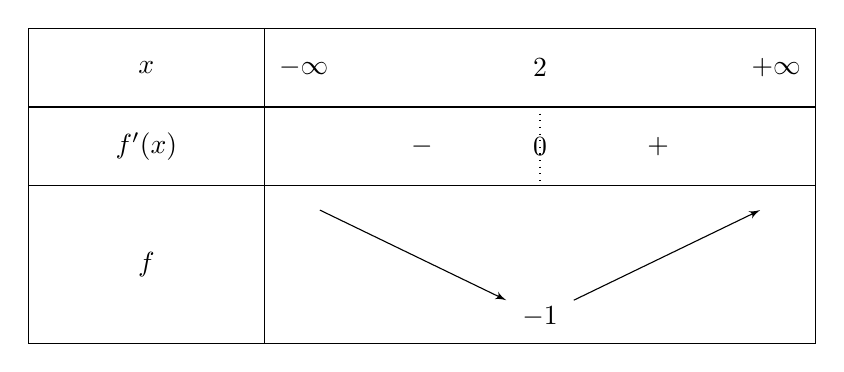
\begin{tikzpicture}
\tkzTabInit[lgt=3,espcl=3]{$x$ /1, $f'(x)$ /1, $f$ /2}{$-\infty$, $2$, $+\infty$}
\tkzTabLine{, -, z, +, }
\tkzTabVar{+/ , -/$-1$, +/ }
\end{tikzpicture}
\end{center}

\subsection*{\underline{\textbf{\textcolor{red}{3. Extremum d'une fonction}}}}
Lorsque la fonction dérivée s'annule en changeant de signe, la fonction admet un \textbf{extremum} (un maximum ou un minimum local).

\underline{\exemple} Dans le tableau ci-dessus, la dérivée change de signe ($- \to +$) en $2$. La fonction atteint donc son minimum en $x = 2$, et ce minimum vaut $f(2) = -1$.

\section*{\underline{\textbf{\textcolor{red}{IV. Applications économiques (Coût et Bénéfice)}}}}

En première L, la dérivation est souvent utilisée pour étudier des fonctions de coûts de production d'une entreprise ou de recettes.

\underline{\exemple}
Une entreprise produit $x$ objets. Le bénéfice réalisé en milliers de francs est donné par la fonction :
\[
B(x) = -x^2 + 8x - 12 \quad \text{pour } x \in [0 ; 10]
\]
1. Calculons le bénéfice dérivé : $B'(x) = -2x + 8$.\\
2. Cherchons pour quelle production le bénéfice est maximal :
\[
B'(x) = 0 \implies -2x + 8 = 0 \implies x = 4
\]
L'entreprise doit produire 4 objets pour obtenir un bénéfice maximal. Ce bénéfice maximum est de $B(4) = -(4)^2 + 8(4) - 12 = -16 + 32 - 12 = 4$ milliers de francs.

\end{document}